\subsection{Metodología de Gestión de Actividades}

La gestión de actividades se articula directamente con SCRUM, el cual fue seleccionado como el marco de trabajo que guía la metodología de desarrollo de software. Bajo este enfoque, el proyecto se organiza en iteraciones semanales fijas, en las que se priorizan tareas, se hace seguimiento al avance y se revisan los entregables definidos para cada \textit{sprint}.

En una primera etapa, la gestión de tareas del proyecto se realizó mediante el tablero Kanban de WebDesk, una plataforma interna de Webcloster utilizada para centralizar distintos procesos operativos de la organización. En este espacio se administraban las actividades del proyecto, se visualizaba el estado de las tareas y se mantenía una trazabilidad básica del trabajo pendiente, en progreso, pausado y finalizado.

\newcommand\webdeskBoardCaption{Tablero Kanban del proyecto en WebDesk, plataforma interna de Webcloster. \hspace{1em}}
\begin{figure}[H]
  \centering
  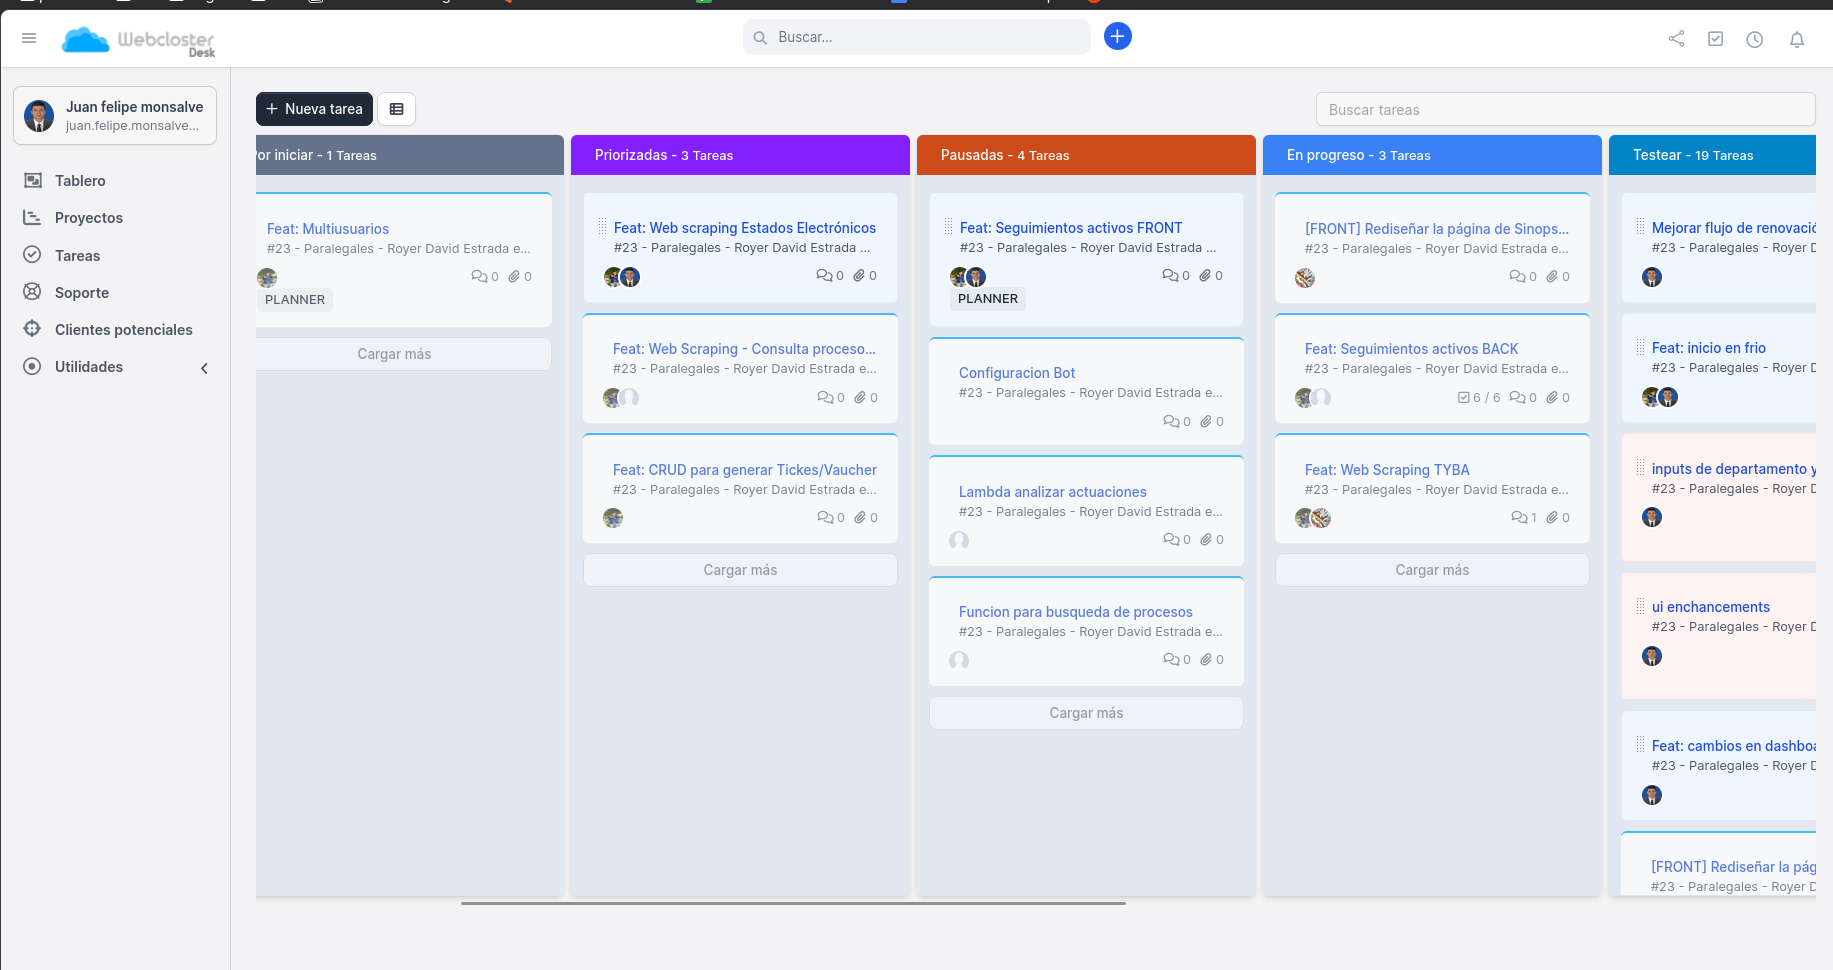
\includegraphics[width=1\textwidth]{uploads/screenshot-2026-05-09_22-07-18.png}
  \caption[\webdeskBoardCaption]{\webdeskBoardCaption Fuente: Elaboración propia.}
  \label{fig:webdesk-kanban}
\end{figure}

Posteriormente, el manejo de tareas migró a Plane, un software \textit{open source} desplegado en modalidad \textit{self-hosted} sobre la infraestructura de Webcloster. Esta transición permitió contar con una herramienta más especializada para la gestión ágil del trabajo, con mejor organización del \textit{backlog}, mayor claridad en los flujos de estado y una administración más robusta de los elementos de trabajo del proyecto.

Dentro de Plane se consolidó el \textit{backlog} del producto y se estructuró el tablero de trabajo del proyecto, facilitando la priorización de funcionalidades y el seguimiento del avance de cada tarea en los distintos estados definidos por el equipo.

\newcommand\planeBoardCaption{Gestión del \textit{backlog} y flujo de trabajo del proyecto en Plane. \hspace{1em}}
\begin{figure}[H]
  \centering
  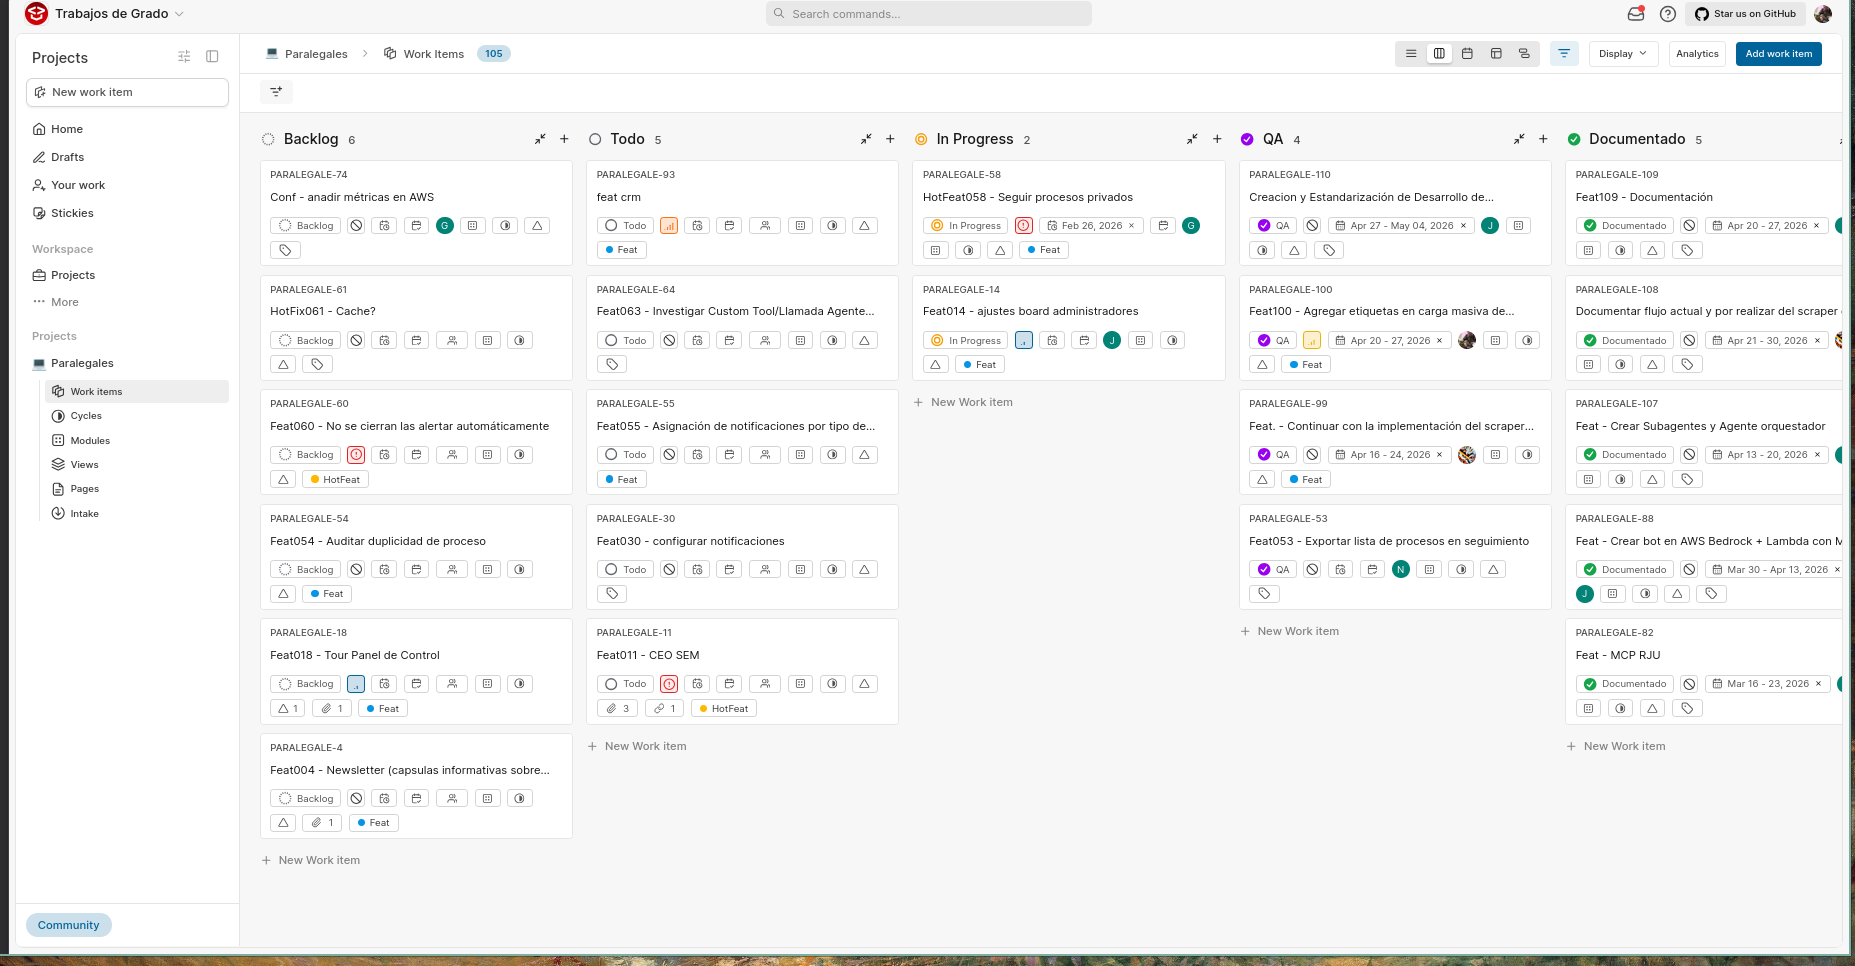
\includegraphics[width=1\textwidth]{uploads/screenshot-2026-05-09_22-00-04.png}
  \caption[\planeBoardCaption]{\planeBoardCaption Fuente: Elaboración propia.}
  \label{fig:plane-board}
\end{figure}

A partir de este \textit{backlog}, se seleccionan las tareas y funcionalidades a priorizar en cada \textit{sprint} mediante reuniones sincrónicas con el equipo de trabajo, conformado por desarrolladores, \textit{Product Owner} y \textit{Tech Lead}. De esta forma, la herramienta de gestión de actividades sirve como soporte operativo para la planeación, ejecución y control continuo del proyecto.

Por otro lado, la comunicación sincrónica se gestiona mediante Google Meet para realizar sesiones de \textit{sprint planning} y mediante Discord para actividades de \textit{pair programming} y revisión de código. En cuanto a la comunicación asincrónica, una parte importante se realiza a través de Telegram, herramienta utilizada para compartir avances, resolver dudas puntuales y recibir notificaciones técnicas del sistema.

\newcommand\telegramDailyCaption{Canal de Telegram utilizado para la comunicación asincrónica del equipo. \hspace{1em}}
\begin{figure}[H]
  \centering
  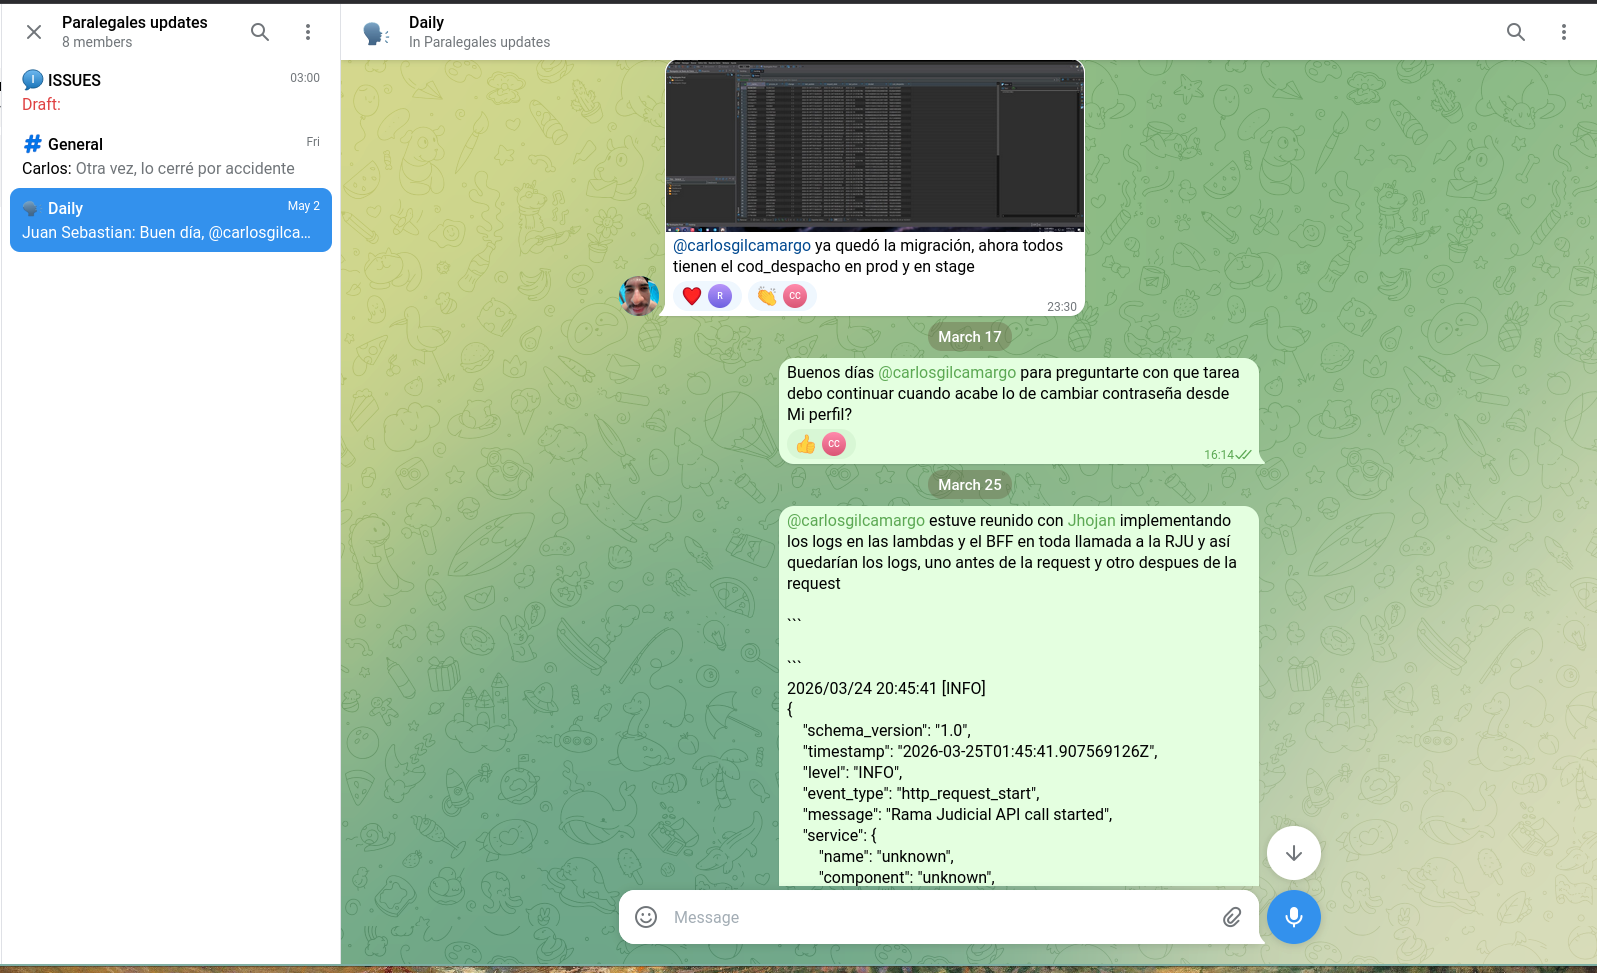
\includegraphics[width=1\textwidth]{uploads/screenshot-2026-05-09_22-01-54.png}
  \caption[\telegramDailyCaption]{\telegramDailyCaption Fuente: Elaboración propia.}
  \label{fig:telegram-daily}
\end{figure}

Además, Telegram también se emplea para la recepción de alertas y notificaciones automáticas asociadas al comportamiento de la plataforma en producción, lo cual contribuye al monitoreo oportuno y a la atención temprana de incidentes.

\newcommand\telegramAlertsCaption{Canal de Telegram usado para recibir alertas automáticas del sistema. \hspace{1em}}
\begin{figure}[H]
  \centering
  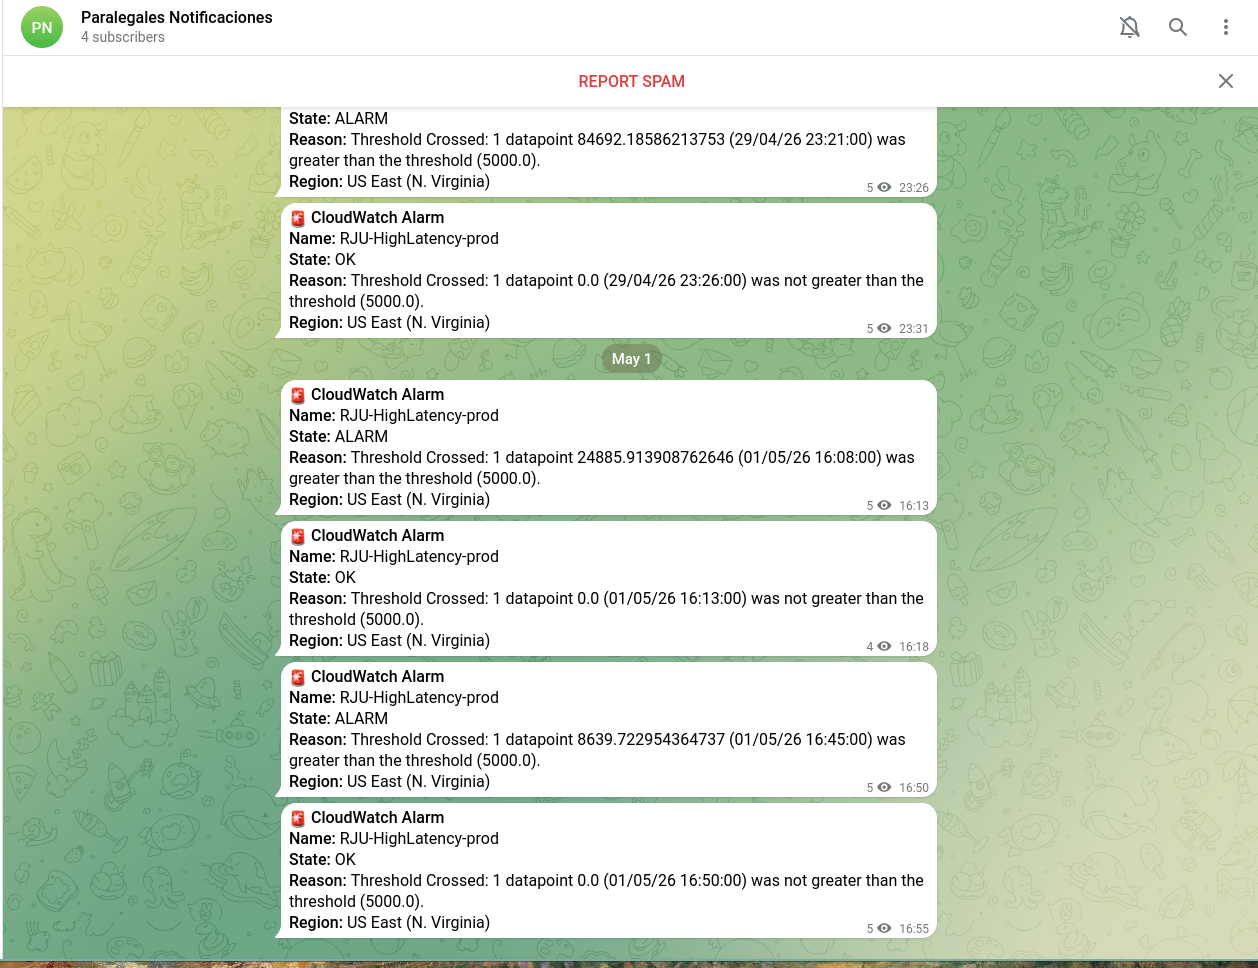
\includegraphics[width=0.72\textwidth]{uploads/screenshot-2026-05-09_22-01-14.png}
  \caption[\telegramAlertsCaption]{\telegramAlertsCaption Fuente: Elaboración propia.}
  \label{fig:telegram-alerts}
\end{figure}
